\section{Introducing Views}
\label{sec.views}


\subsection{Practical genericity for efficiency: the Views}
\label{subsec.views}

Let us introduce another key point enabled by genericity and concepts: the \emph{Views}. A \emph{View} is defined by a
non-owning lightweight image, inspired by the design introduced in \emph{Ranges for the Standard
  Library}~\citep{niebler.2014.ranges} proposal for \emph{non-owning collections}. A similar design is also called
\emph{Morphers} in \textsc{Milena}~\citep{levillain.2009.ismm, geraud.2012.hdr}. \emph{Views} feature the following
properties: \emph{cheap to copy}, \emph{non-owner} (does not \emph{own} any data buffer), \emph{lazy evaluation}
(accessing the value of a pixel may require computations) and \emph{composition}. When chained, the compiler builds a
\emph{tree of expressions} (or \emph{expression template} as used in many scientific computing libraries such as
Eigen~\cite{guennebaud.2010.eigen}), thus it knows at compile-time the type of the composition and ensures a 0-overhead
at evaluation.

There are four fundamental kind of views, inspired by functional programming paradigm: \texttt{transform(input, f)}
applies the transformation $f$ on each pixel of the image \emph{input}, \texttt{filter(input, pred)} keeps the pixels of
\emph{input} that satisfy the predicate \emph{pred}, \texttt{subimage(input, domain)} keeps the pixels of \emph{input}
that are in the domain \emph{domain}, \texttt{zip($input_1$, $input_2$, \ldots, $input_n$)} allows to pack several pixel
of several image to iterate on them all at the same time.

\emph{Lazy-evaluation} combined with the view \emph{chaining} allows the user to write clear and very efficient code
whose evaluation is delayed till very last moment as shown in~\cref{fig.lazy} (see \cite{geraud.2018.gtgdmm} for
additional examples). Neither memory allocation nor computation are performed; the image $i$ has just recorded all the
operations required to compute its values.

\begin{figure}[htbp]
  \begin{minipage}[l]{0.48\linewidth}
    \begin{minted}{C++}
image2d<rgb8>  ima1 = /* ... */;
image2d<uint8_t> ima2 = /* ... */;

// Projection: project the red channel value
auto f = view::transform(ima, [](auto v) {
  return v.r;
});

// Lazy-evaluation of the element-wise
// minimum
auto g = view::transform(view::zip(f, ima2),
  [](auto value) {
    return std::min(std::get<0>(value),
             std::get<1>(value));
});
\end{minted}
  \end{minipage}
  \hfill
  \begin{minipage}[l]{0.48\linewidth}
    \begin{minted}{C++}
// Lazy-Filtering: keep pixels whose value
// is below < 128
auto h = view::filter(g, [] (auto value) {
  return value < 128;
}));

// Lazy-evaluation of a gamma correction
using value_t = typename Image::value_type;
constexpr float gamma = 2.2f;
constexpr auto max_val =
  std::numeric_limits<value_t>::max();
auto i = view::transform(h,
  [gamma_corr = 1 / gamma] (auto value) {
    return std::pow(value / max_val,
             gamma_corr) * max_val;
});
\end{minted}
  \end{minipage}

  \caption{Lazy-evaluation and \emph{view} chaining.}
  \label{fig.lazy}
\end{figure}

\noindent The tree of type resulting from this view chaining is illustrated by~\cref{fig.viewAST}.

\begin{figure}[htb]
  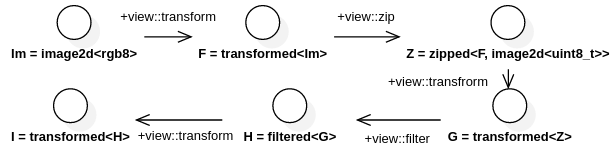
\includegraphics[height=2cm]{figs/viewAST.png}
  \caption{Abstract Syntax Tree of the types chained by the code above}
  \label{fig.viewAST}
\end{figure}

The concept of \emph{View} brought to us a fundamental issue when dealing with images: \blockquote{\emph{What is an
    image?}}. More precisely: should an image always be the owner of its data buffer? Should we have a shared ownership of
the data buffer between all the images using it? Then what happens when the data changes? The issue about the semantic
of an image is crucial but also very similar to the issue there is to differentiate a \emph{container} (such as
\texttt{std::vector}, that is to say the data buffer) and a \emph{view} on this container in the \emph{Ranges TS}.

From here we have considered two approaches. The first one is to have \emph{shared ownership} of the data buffer for the
image and its derived views. However this does not allow the differentiation between an already computed image and a
lazy image. To be able to make this differentiation is crucial in an \emph{Image Processing library} as we want to make
the most out of the data we already have and we do not want to compute data we do not need. Also, we cannot distinguish
when the \emph{copyability} property is required. This is the main reason why we did not adopt this approach.

The second one is to make the differentiation between a \emph{concrete image} which owns the data (like the standard
containers) and the \emph{views} that are lightweight cheap-to-copy objects. Not all \emph{concrete image} may be
\emph{copyable}, but all \emph{views} are. This is a very important property as it simplify greatly the reasoning when
performance is needed. It also enables us to have a library design similar to the standard library which the user is
familiar with and, why not, have standard algorithm and standard view work on our images types. All of these are the
main reason why we decided to adopt this design. Henceforth from now on the \emph{Image} concept is similar to the
\emph{View} concept from which we refines a \emph{ConcreteImage} concept that requires a specific behavior as it owns
data.


\vspace{1cm}

In~\cref{subsec.gen.concept}, we saw that what is truly important is the behavior: an algorithm will require its input
to be able to behave a certain way, and if those requirements are fulfilled, then the algorithm can be used with this
set of inputs. This enables non-standard type of image to be input in algorithms, providing they still behave correctly.
The way how we can check if the required behavior is satisfied is a new C++20 feature called \emph{concept} (the authors
show how to leverage them in~\cite{roynard.2019.rrpr}) that will not be presented in this paper. Additionally to
concepts, C++20 introduces a new library facility called \emph{ranges}~\cite{niebler.2018.deepranges} which includes a
non-owning lightweight container called \emph{views} whose design is very similar to that of \emph{morphers}, introduced
in Milena~\cite{levillain.2009.ismm,geraud.2012.hdr}. Views are completely transferable to the image processing world.
Also, views feature interesting properties that an image processing practitioner will find to his taste.

A view is a \emph{lightweight object} that behaves exactly the same as an image: let $V$ be a view of an image defined
on $\mathcal{D}$ then we have $\forall{p}\in\mathcal{D}, v = V(p)$. It can be a random generator that yields a random
number each time $V(p)$ is called; a proxy to the underlying image that records the number of times each pixel is
accessed in order, for instance, to compare algorithm performance; a projection to a specific color channel; applying an
automatic gamma correction; restricting the definition domain $\mathcal{D}$; and so on.

A view is a \emph{non-owning}, \emph{cheap-to-copy} lightweight object that basically only \emph{records an operation}
and stores a pointer to an image. For instance, let us consider the view transform defined as follow $v = transform(u_1,
  u_2, \cdots, u_n, f)$ where $u_i$ are input images and $h$ a n-ary function. $transform$ returns an image generated from
the other image(s) as show in~\cref{fig.view.threshold}. Also, we can see that the view itself does not own any image
but just stores pointers as well as the operation ($h$). This means that, for instance, modifying the original values of
the image(s) will impact the values yield by the view. Finally, as the view is cheap-to-copy, it features a pointer
semantic that help the practitioner passing around his images by copy to his algorithms without worrying about heavy
buffer copies in the background.

\begin{figure}[tbh]
  \centering
  \begin{minipage}{\linewidth}
    \includestandalone[mode=image, width=.9\linewidth]{figs/transform_thresholding}
  \end{minipage}
  \caption{An image view performing a thresholding.}
  \label{fig.view.threshold}
\end{figure}

Another key point of views is the lazy evaluation. When an image is piped through a view, no computation is done. The
computation happens when the practitioner requests a value by doing $val = V(p)$. The implications are multiples: an
image can be piped into several computation-heavy views, some of which can be discarded later on, it won't impact the
performance. Also, when processing large images, applying a transformation on a part of the image is as simple as
restricting the domain with a view and applying the transformation to this resulting sub-image.

Views will also try to preserve properties of the original image when they can. That means that views can preserve the
ability of the practitioner to, for instance, write into this image. This may be a trivial property to preserve when
considering a view that restrict a domain, but when considering a view that transforms the resulting values, it is not.
Let us consider the projection $h: (r,g,b) \mapsto g$ that selects the green component of an RGB triplet. When piping
the resulting view into, for instance, a blurring algorithm, the computation will take place in place thanks to still
having the ability to write into the image. A legacy way of obtaining the same result would have been to create a
temporary single-channel image consisting of the green channel of the original RGB image so that the temporary image
could then be blurred. Then one would have needed to copy the values of the temporary image back into the green channel
of the original image. The comparison between the legacy way and the in-place way of doing this computation is shown
in~\cref{fig.legacy.vs.view}.

\begin{figure}[tbh]
  \centering
  \subfloat[Legacy pipeline with copy]{
    \includegraphics[width=1.6in,align=t]{figs/blur_copy}
  }
  \hfil
  \subfloat[Modern pipeline with view]{
    \includegraphics[width=1.6in,align=t]{figs/blur_inplace}
  }

  \caption{Comparison of a legacy and a modern pipeline using \colorbox{lightgreen}{algorithms} and
    \colorbox{thistle}{views}.}
  \label{fig.legacy.vs.view}
\end{figure}

On the other hand, when considering the view $g: (r,g,b) \mapsto 0.2126*r+0.7152*g+0.0722*b$ that compute the gray level
of a color triplet (as shown in~\cref{fig.view.grayscale}), the ability to write a value into the image is not
preserved. One would need an inverse function that is able to deduce the original color triplet from the gray level to
be able to write back into the original image.

\begin{figure}[tbh]
  \centering
  \includegraphics[width=.98\linewidth]{figs/views/transform_grayscale}
  \caption{Usage of transform view: grayscale.}
  \label{fig.view.grayscale}
\end{figure}

\begin{figure}[tbh]
  \includestandalone[mode=image, scale=0.6]{figs/clip}

  \includestandalone[mode=image, scale=0.6]{figs/filter}
  \caption{Clip and filter image adaptors that restrict the image domain by a non-regular ROI and by a predicate that
    selects only even pixels.}
  \label{fig.view.clip}
\end{figure}

Following the same principle, a view can apply a restriction on an image domain. In~\cref{fig.view.clip}, we show the
adaptor \texttt{clip(input, roi)} that restricts the image to a non-regular \texttt{roi} and \texttt{filter(input,
  predicate)} that restricts the domain based on a predicate. All subsequent operations on those images will only affect
the selected pixels.

\begin{figure}[tbh]
  \includestandalone[mode=image, scale=0.6]{figs/pipeline}
  \caption{Example of a simple image processing pipeline.}
  \label{fig.view.pipeline}
\end{figure}

Views feature many interesting properties that change the way we program an image processing application. To illustrate
those features, let us consider the following image processing pipeline: (Start) Load an input RGB-8 2D image (a
classical HDR photography) (A) Convert it in grayscale (B) Sub-quantize to 8-bits (C) Perform the grayscale dilation of
the image (End) Save the resulting 2D 8-bit grayscale image; as described in~\cref{fig.view.pipeline}.


\begin{figure}[tbh]
  \begin{minipage}{\linewidth}
    \includestandalone[mode=image, scale=0.59]{figs/composition}
  \end{minipage}
  \caption{Algorithm vs image view composition.}
  \label{fig.view.comp}
\end{figure}

\textbf{Views are composable.} Chaining operations has always been a very important feature in image processing as well
as in software engineering in general (known object composition). Being able to weave simple blocks together into more
complex blocks in a way that the resulting block can still be treated as a simple block is a most wanted feature.
The~\cref{fig.view.pipeline} features an example of a pipeline using 3 basic operations \emph{Image} $\rightarrow$
\emph{Image}: a grayscale conversion, a sub-quantization and a dilation. It is important to note that we can consider
there is only one complex operation composed of 3 basic algorithms in which an image is piped. A view thus carries both
information about the image and the transformations. In~\cref{fig.view.comp} we show the distinction between the
composition of algorithms and the compositions of views which carry both the image and the transformations.

\textbf{Views improve usability.} The code featuring the pipeline in~\cref{fig.view.comp} can almost be implemented the
following way:
\begin{minted}{c++}
auto input = imread(...);
auto A = transform(input, [](rgb16 x) -> float {
    return (x.r + x.g + x.b) / 3.f; };
auto MyComplexImage = transform(A, [](float x)
    -> uint8_t { return (x / 256 + .5f); };
\end{minted}
When one is familiar to functional programming, it is quite easy to draw the parallel between \emph{transform},
\emph{map}, \emph{filter} and the sequence operators. Views are, in reality, higher-order functions built from an image
as well as the function(s) (operator or predicate) to apply for each pixel. It is not required to make the iteration
over each pixel of the image oneself, we just provide the function to morph the image into another one. The technique
used when composition several sequence operators is called \emph{currying}~\cite{hanus.1995.curry} in the functional
programming world.

\textbf{Views improve re-usability.} When looking at the code snippets above, one could see that they are simple though
not very re-usable. However, keeping the functional programming paradigm in mind, one can easily define new views just
by considering that a view is a \emph{higher-order function}. Then, as shown in~\cref{fig.view.highorder}, the primitive
\emph{transform} serves as the basis to build three new views: one that performs the summation of two images, one that
performs the grayscale conversion and one that performs the sub-quantization. All those three views can then be reused
afterwards\footnote{A more generic implementation could have been provided for these views for even more re-usability,
  but this is not the purpose here.}.

\begin{figure}
  \noindent
  \begin{minted}{c++}
auto operator+(Image A, Image B) {
  return transform(A, B, std::plus<>());
}
auto togray = [](Image A) { return transform(A, [](auto x)
  { return (x.r + x.g + x.b) / 3.f; };)
};
auto subquantize16to8b = [](Image A) { return transform(A,
  [](float x) { return uint8_t(x / 256 +.5f); });
};

auto input = imread(...);
auto MyComplexImage = subquantize16to8b(togray(A));
  \end{minted}

  \caption{Using high-order primitive views to create custom view operators.}
  \label{fig.view.highorder}
\end{figure}

\textbf{Views for lazy computing.} One fundamental point of views is that they embed the operation within themselves,
meaning that in~\cref{fig.view.highorder}, the creation of the views does not incur any computation. The computation is
delayed until the invocation of the \texttt{v(p)} expression. Also, the computation can be delayed quite far thanks to
the composition capability of views. In fact, a view is an image adaptor which actually is a \emph{template
  expression}~\citep{veldhuizen.1995.expression, veldhuizen.2000.blitz}. Indeed, the \emph{expression} used to generate
the image is recorded as a template parameter. A view is represented by an \emph{expression tree}, as shown
in~\cref{fig.view.ast}.


\begin{figure}
  \null\hfill
  \begin{minipage}[b]{2cm}
    \includestandalone[mode=image, scale=0.8]{figs/view_ast}
  \end{minipage}
  \begin{minipage}[b]{5.5cm}
    \begin{minted}{c++}
Image f = ...; // grayscale
Image g = ...; // rgb16
Image out = subquantize16to8b(
              togray(g)) + f;
\end{minted}
  \end{minipage}
  \caption{View composition seen as an expression tree.}
  \label{fig.view.ast}
\end{figure}



\PLAGIAT{
  \textbf{Views for performance.} Consider a classical design where each operation of the pipeline is implemented on
  ``its own''. Each operation requires that memory be allocated for the output image, and also, each operation requires
  that the image be traversed. This design is simple, flexible, composable, but is not memory efficient nor
  computationally efficient. With the lazy evaluation approach, the image is traversed only once (when the dilation is
  applied) that has two benefits. First, there are no intermediate images so this is memory effective. Second, it is
  faster thanks to a better memory cache usage; processing a RGB16 pixel from the dilation algorithm directly converts
  it in grayscale, then sub-quantized it to 8-bits, and finally make it available. It acts \emph{as if} we were writing
  an optimal operator that would combine these operations.
}

\PLAGIAT{
  As an experiment, we benchmarked both pipelines on a 20MPix image RGB16 (random generated values) on a desktop
  computer i7-2600 CPU @ 3.40GHz, single-threaded\footnote{Experimentation code is available at
    \url{https://gitlab.lrde.epita.fr/mroynard/roynard.icip.2020.snippets}}. The dilation is done with a small 3x3 square
  structuring element using tiling for caching input values. The pipeline using views is about 20\% faster than the
  regular one (133 vs 106 ms). Note that views are also compatible with optimizations such as parallelization and
  vectorization.
}

\PLAGIAT{
  Background Subtraction: The background subtraction pipeline is used to detect changes in image
  sequences~\cite{opencv.bg_sub}. It is mainly used when regions of interest are foreground objects. The pipeline
  components include: subtraction, Gaussian filtering, threshold, erode and dilate, as shown
  in~\cref{fig.view.comp.sub_bg}.
}

\begin{figure}[tbh]
  \begin{minipage}{\linewidth}
    \includestandalone[mode=image, scale=0.59]{figs/pipeline_bg_sub_comp}
  \end{minipage}
  \caption{Background substraction pipeline using \colorbox{lightgreen}{algorithms} and
    \colorbox{thistle}{views}.}
  \label{fig.view.comp.sub_bg}
\end{figure}


\clearpage


\begin{itemize}
  \item origine, parallèle avec range-v3
  \item Value/Ref semantics des images
  \item Comment préserver les propriétés
  \item Évaluation paresseuse
  \item Composabilité/chaînage
  \item ...
  \item Performances + Bench
\end{itemize}